% 函数增量示意图
\begin{figure}[htbp]
  \centering
  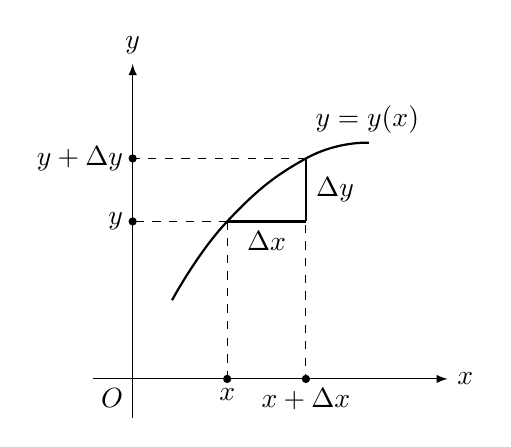
\begin{tikzpicture}
    \draw[-latex] (-0.5,0) -- (4,0) node[right] {$x$};
    \draw[-latex] (0,-0.5) -- (0,4) node[above] {$y$};

    \node[below left] at (0,0) {$O$};

    \coordinate (A) at (1.2,2);
    \coordinate (B) at (2.2,2.8);

    \draw[thick]
        plot[smooth,tension=0.8] coordinates {
          (0.5,1)
          (A)
          (B)
          (3,3)
        };

    \node[above right] at (B|-0,3) {$y = y(x)$};

    \draw[dashed] (A) -- (A|-0,0) node[below] {$x$};
    \draw[dashed] (B) -- (B|-0,0) node[below] {$x + \Delta x$};

    \draw[dashed] (A) -- (0,0|-A) node[left] {$y$};
    \draw[dashed] (B) -- (0,0|-B) node[left] {$y + \Delta y$};

    \draw[-,thick] (A) --(B|-A) node[midway,below] {$\Delta x$};
    \draw[-,thick] (B|-A) --(B) node[midway,right] {$\Delta y$};
    

    \fill (A|-0,0)circle [radius=1.5pt]
          (B|-0,0)circle [radius=1.5pt]
          (0,0|-A)circle [radius=1.5pt]
          (0,0|-B)circle [radius=1.5pt];
  \end{tikzpicture}
  \caption{}
  \label{fig:function-increment}
\end{figure}
